\chapter{Aufgabe 2:  Recherche von aktuellen Angriffsszenarien}

\section{a)}

\textit{Recherchieren Sie im Internet bzgl. aktueller Angriffe auf IT‐Systeme und sicher‐
heitsrelevanter Meldungen, die in den letzten Monaten stattgefunden haben, und geben Sie fünf der gefundenen Angriffe bzw. Meldungen an. }

\vspace{5mm}

\begin{itemize}
    \itemsep0.5em
    \item \textbf{Bybit-Hack} Im Februar 2025 wird die Kryptobörse \textit{Bybit} Opfer eines Hacks, bei dem über 1.5 Milliarden Dollar von nordkoreanischen Hackern erbeutet werden\footnote{
    \url{https://announcements.bybit.com/en/article/incident-update-unauthorized-activity-involving-eth-cold-wallet-blt292c0454d26e9140/}, abgerufen 23.03.2025
    }. Es berichten u.a. Telepolis\footnote{
        \url{https://www.telepolis.de/features/Groesster-Krypto-Diebstahl-aller-Zeiten-Nordkorea-klaut-1-5-Milliarden-Dollar-bei-Bybit-10295169.html}, abgerufen 23.03.2025
    } sowie Spiegel.de \footnote{
        \url{https://www.spiegel.de/netzwelt/web/bybit-nordkoreas-hacker-sollen-milliarden-bei-kryptoboerse-erbeutet-haben-a-529d2692-6be9-4f4b-965f-7b192c7c6f2a}, abgerufen 23.03.2025
    }.
    \item \textbf{Storm-0408} Microsoft berichtet im März 2025\footnote{
    \url{https://www.microsoft.com/en-us/security/blog/2025/03/06/malvertising-campaign-leads-to-info-stealers-hosted-on-github/}, abgerufen 23.05.2025
    } von einem Malware-Angriff über (illegale) Streamingseiten, bei denen eingebettete Werbeanzeigen Schadsoftware auf den Rechner der Benutzer installieren.
    \item \textbf{DDOS-Angriff X.com} Wired.com berichtet im März 2025\footnote{
    \url{https://www.wired.com/story/x-ddos-attack-march-2025/}, abgerufen 23.03.2025
    }über eine Distributed-Denial-of-Service-Attacke gegen X.com (ehemals twitter.com).

    \item \textbf{Fortinet Zero-Day exploit} In einer Warnmeldung vom Januar 2025 berichtet das BSI\footnote{
        \url{https://www.bsi.bund.de/SharedDocs/Cybersicherheitswarnungen/DE/2025/2025-213432-1032.pdf?__blob=publicationFile&v=2}, abgerufen 23.03.2025
    } von einer Zero-Day-Schwachstelle bei FortiOS und FortiProxy, durch die Angreifer Super-Admin-Privilegien erlangen können.
    \item \textbf{Sicherheitsgefahr durch EOL-Versionen von MS Exchange} das BSI berichtet im März 2025\footnote{
    \url{https://www.bsi.bund.de/SharedDocs/Cybersicherheitswarnungen/DE/2024/2024-223466-1032.pdf?__blob=publicationFile&v=7} ,abgerufen 23.03.2025
    } von Sicherheitslücken bei Versionen von MS Exchange Servern, die offiziell keinen Support mehr erfahren (\textit{End-of-Life}), aber trotzdem noch von Institutionen betrieben werden.
\end{itemize}

\section{b)}
\textit{Beschreiben Sie die prinzipielle Vorgehensweise des Angreifers für zwei der in a) angegebenen Angriffe (jeweils maximal eine Seite Text, inkl. Abbildungen!).}


\subsection*{DDOS-Angriff X.com}

\begin{itemize}
    \itemsep0.5
    \item Betroffenes Schutzziel: \textbf{Verfügbarkeit}
    \item Maßnahmen: u.a. \textbf{Entkoppelung}, \textbf{Skalierung d. Infrastruktur}, \textbf{IPS}\footnote{
    \textit{Intrusion Prevention System}: System zur Analyse von Netzwerkverkehr (NBA - \textit{Network Behavior Analysis}) zur Erkennung verschiedener Angriffsformen
    }
\end{itemize}
\noindent
X.com nutzt die Dienste von Cloudflare\footnote{
\url{https://cloudflare.com}, abgerufen 23.03.2025
}, um sich gegen DDOS-Attacken zu schützen\footnote{
Hinweis im o.a. Artikel, weitere Hinweise liefern aber auch bspw. DNS-Anfragen, die im A-Record auf eine CloudFlare-IP (172.66.0.227) verweisen (letzter Zugriff 23.03.2025)
}.\\
Bei DDOS-Angriffen (Distributed-Denial-of-Service) handelt es sich um Angriffe, die einen Dienst mit Anfragen überhäufen, bis die technischen Kapazitäten der Infrastruktur erschöpft sind und keine Anfragen mehr beantwortet werden können (vgl.~\cite[120 ff.]{Eck18} sowie~\cite[533 ff.]{SL05}).\\
Als schwierig erweist sich hierbei i.d.R. eine erfolgreiche Unterscheidung regulärer von maliziösen Anfragen, da Anfragen verteilt (\textit{distributed}) aus verschiedenen IP-Netzen versendet werden.
Ein einzelner Angreifer kann also nicht ausgemacht werden.
Das Prinzip ist in Abbildung~\ref{fig:ddos} dargestellt.\\


\begin{figure}
    \centering
    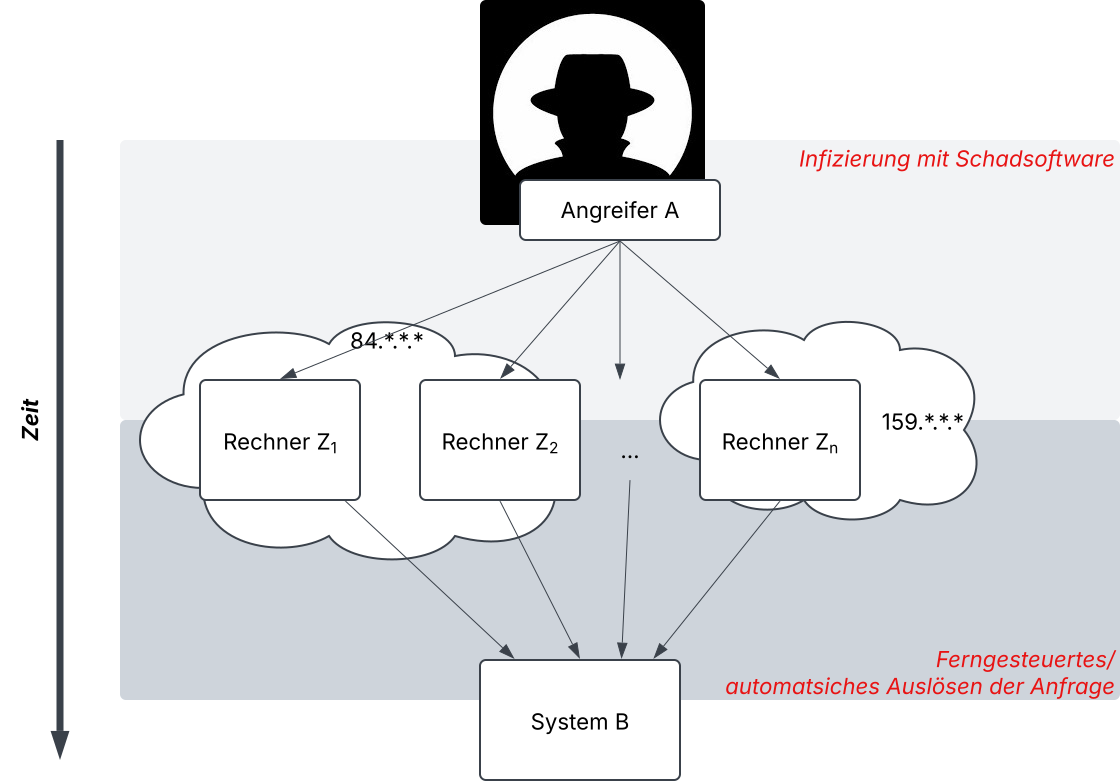
\includegraphics[scale=0.3]{aufgabe 2/img/ddos.svg}
    \caption{Vereinfachte Darstellung eines DDOS-Angriffes. Angreifer A nutzt Schadsoftware, um die Rechner $Z_1, Z_2 \ldots, Z_n$ zu infizieren. Die Schadsoftware  instruiert die Rechner - nun Teilnehmer eines Botnetzes - zu einem bestimmten Zeitpunkt Anfragen an eine bestimmtes Zielsystem B zu senden. In Summe führt dies zu der Überlastung des Angriffsziels. Anfragen können nicht mehr abgearbeitet werden, der Dienst steht nicht mehr zur Verfügung. (Quelle: eigene)}
    \label{fig:ddos}
\end{figure}


\noindent
Es wird deshalb oft auf Dienstleister zurückgegriffen, die technische Kapazitäten zur Bereitstellung großer Server-Infrastrukturen besitzen und diese gleichzeitig darauf ausrichten, Angriffen solcher Art entgegenzuwirken.
Für Institution bedeutet solch ein Vorhaben ansonsten hohen personellen und technischen Aufwand.\\

\noindent
wired.com zitiert bzgl. des Angriffs \textit{Kevin Beaumont}\footnote{
    \url{https://doublepulsar.com/}, abgerufen 23.03.2025
}, der das Botnetz als einen Verbund aus Kameras und DVRs beschreibt, also IoT-Geräten, die im Kontext ``Sicherheitsniveau`` oft nur unzureichend berücksichtigt werden, wie \textit{Münch und Schnaumüller-Bichl} in  (\cite[36]{ITS2}) anmerken.\\
In diesem Fall war die Sicherheitslücke anscheinend durch den Umstand begünstigt, dass einige der Dienste von X.com nicht durch die Infrastruktur von CloudFlare geschützt gewesen sind:

\blockquote[]{
``[\ldots] some X origin servers, which respond to web requests, weren't properly secured behind the company's Cloudflare DDoS protection and were publicly visible.``
}